\section{Ejercicios resueltos}
\subsection{Tema 1: Fundamentos y propiedades de los fluidos}
\begin{enumerate}
	\item Obtener el ángulo de mojabilidad $\theta_c$ 
	\begin{figure}[H]
		\begin{minipage}{0.7\textwidth}
		\centering
		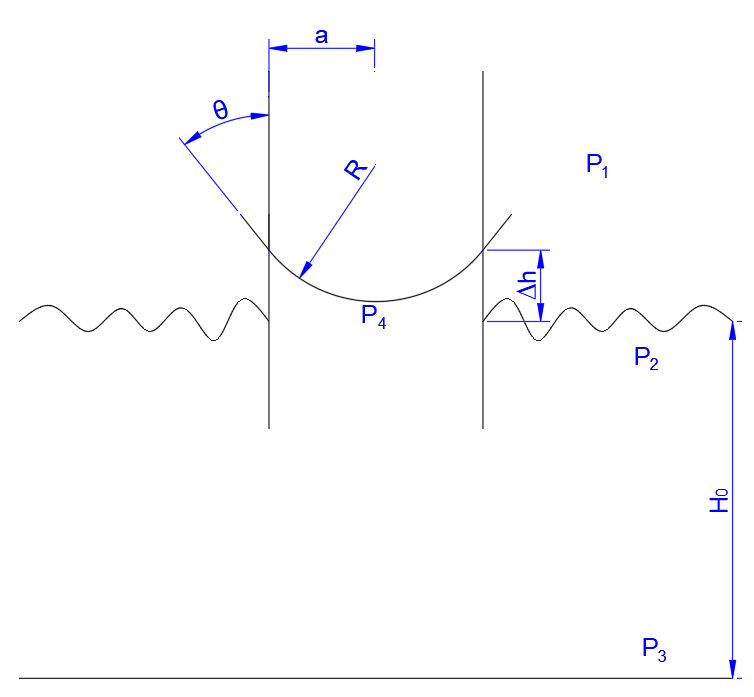
\includegraphics[width=0.7\linewidth]{imagenesEjercicios/mojabilidad}
		\caption{Esquema del problema.}
		\label{fig:mojabilidad}
	\end{minipage}%
	\begin{minipage}{0.3\textwidth}
	\[\textcolor{red}{P_2=P_1=P_a}\]
	\[\textcolor{red}{P_2=\rho g H_0=P_3}\]
	\[\textcolor{red}{P_3=P_4+\rho g (H_0+\Delta h)}\]
	\[\textcolor{red}{P_1-P_4=\frac{2\sigma}{R}}\]
	\[\textcolor{red}{\frac{2\sigma}{R}=\rho g \Delta h}\]
	\[\textcolor{red}{Rcos(\theta_c)=a}\]
	\[\textcolor{red}{\theta_c=arccos\left(\frac{a\rho g \Delta h}{2\sigma}\right)}\]
	
	\end{minipage}
	\end{figure}
	
	\item En el pueblo de Aisa se ha instalado un nuevo sistema de presión para el abastecimiento
	de agua del municipio. El agua procedente de un manantial es impulsado por una bomba
	y se almacena en un depósito sobrepresor. Para controlar la presión del agua a la entrada
	y salida de la bomba se han montado un vacuómetro y un manómetro en los puntos de
	interés. Cuando el vacuómetro marca 0.75 bares y el manómetro marca 4.2 bares, ¿cuál
	será el valor de la presión absoluta?. ¿Existe riesgo de cavitación en algún punto de la
	conducción?. Datos: $p_{atm}$ = 816,91 hPa; $p_v$=159856 Pa.
	\begin{figure}[H]
		\begin{minipage}{0.7\textwidth}
		\centering
		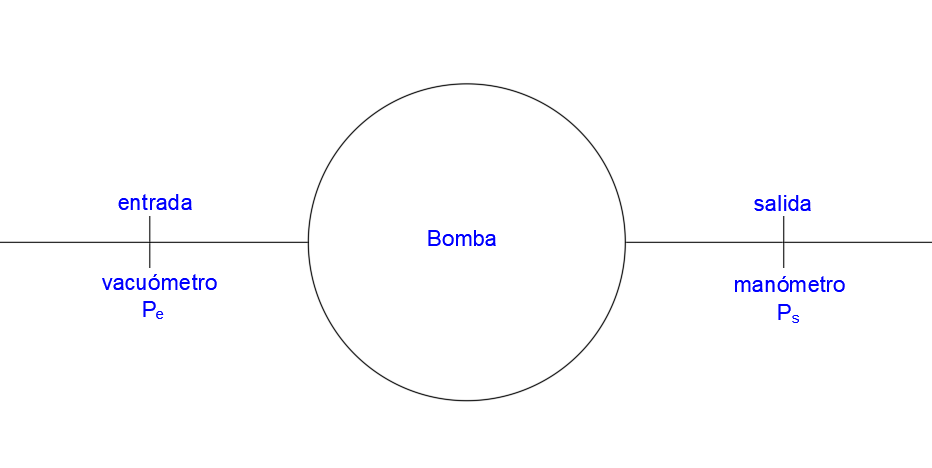
\includegraphics[width=0.7\linewidth]{imagenesEjercicios/bombaAisa}
		\caption{Esquema bomba de agua.}
		\label{fig:bombaaisa}
	\end{minipage}%
	\begin{minipage}{0.3\textwidth}
	\[\textcolor{red}{P_v=P_{atm}-P_e}\]
	\[\textcolor{red}{P_m=P_s-P_{atm}}\]
\[ \textcolor{red}{P_e=81691-75000=6691 Pa}\]
\[\textcolor{red}{P_s=81691+420000=501691 Pa}\]
\textcolor{red}{Existe cavitación a la entrada.}
	
	\end{minipage}
\end{figure}

	\newpage
	\item La presión en un punto de un fluido ($\rho = 1234 \frac{kg}{m^3}$) alcanza el valor de 3 bares. Expresar
	el valor de la presión en milímetros de mercurio (cm Hg) y en columna de metros de agua
	(m.c.a.). Datos: $\rho_{Hg,rel} = 13,6$
	\[\textcolor{red}{\rho = 1234 \frac{kg}{m^3}}\]
	\[\textcolor{red}{P=3\cdot10^5 Pa}\]
	\[\textcolor{red}{1mmHg=\rho_{Hg}g h=13.6\cdot10^3\frac{kg}{m^3} \cdot9.8 \frac{m}{s^2}\cdot10^{-3}m=133.416Pa} \]
	\[\textcolor{red}{1mca=\rho_{H_2O}g h=10^3\frac{kg}{m^3}\cdot9.8 \frac{m}{s^2}\cdot1m=9810Pa}\]
	\item Sobre una superficie de 4000 $cm^2$, orientada en el espacio por su vector normal $\vec{n}=\vec{k}$, está
	actuando una fuerza$\vec{F}=2\vec{i}+3\vec{j}-3\vec{k}$ (N). Calcular la componente normal de la fuerza y
	la presión que está soportando la superficie
		\[\textcolor{red}{S=4000 cm^2=0.4 m^2}\]
	\[\textcolor{red}{\vec{n}=\vec{k}}\]
	\[\textcolor{red}{\vec{F}=2\vec{i}+3\vec{j}-3\vec{k} \rightarrow F_n=3N}\]
	\[\textcolor{red}{P=\frac{F_n}{S}=\frac{3 N}{0.4 m^2}=7.5Pa}\]
	
	\item Sabiendo que un fluido tiene una densidad de 0.627 $\frac{kg}{l}$ y que su coeficiente de viscosidad
	absoluta es 1.2 cP, calcular su viscosidad cinemática. ¿Cuál es su densidad relativa si
	consideramos el agua como fluido de referencia?. Datos $\rho_{agua} = 999,8\frac{kg}{m^3}$
\[\textcolor{red}{\nu = \frac{\mu}{\rho}=\frac{1.2 cP \cdot \frac{10^{-3} Pa \cdot s}{1 cP}}{0.627 \frac{kg}{l}\cdot\frac{10^3 l}{m^3}}=1.91\cdot10^{-6}\frac{m^2}{s}}\]
\[\textcolor{red}{\rho_{rel}=\frac{\rho}{\rho_{H_2O}}=\frac{0.627 \frac{kg}{l}\cdot\frac{10^3 l}{m^3}}{999.8 \frac{kg}{m^3}}=6.27\cdot10^{-1}}\]
	
	\newpage
	\item En la Figura se muestra un bloque, de bases paralelas con dimensiones 0,3 m x 0,6
	m y altura 0,1 m, de densidad 1800 $\frac{kg}{m^3}$, que desliza con una velocidad constante de
	1 $\frac{m}{s}$ a la largo de un plano inclinado debido a la acción de las fuerzas gravitacionales
	tangenciales al mismo. Entre dicho plano y el bloque hay una película de aceite de espesor
	1 mm. Aplicando equilibrio de fuerzas, calcular la viscosidad del aceite en Po.
	\begin{figure}[H]
		
		\centering
		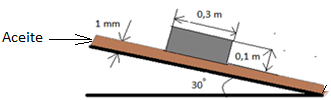
\includegraphics[width=0.7\linewidth]{imagenesEjercicios/bloqueDeslizantoT1}
		\caption{Esquema del bloque deslizando por el plano inclinado.}
		\label{fig:bloquedeslizantot1}
	\end{figure}
	\[\textcolor{red}{F_n=m g sen\alpha}\]
	\[\textcolor{red}{F_n=\rho V g sen\alpha}\]
	\[\textcolor{red}{\tau=\mu\frac{v}{e}=\frac{F_n}{S}=\rho h g sen\alpha}\]
	\[\textcolor{red}{\mu=\frac{e\rho h g sen\alpha}{v}=\frac{10^-3m\cdot1800\frac{kg}{m^3}\cdot0.1m\cdot 9.81 \frac{m}{s^2} \cdot sen(\ang{30})}{1\frac{m}{s}}=0.8829Pa\cdot s\frac{1 P}{0.1 Pa \cdot s}=8.83P}\]
\end{enumerate}
\subsection{Tema 2: Cinemática de la partícula fluida}
\begin{enumerate}
	\item Dado el campo de velocidades de un flujo
	\[\vec{v}=4cos(\omega t)x\vec{i}-2cos(\omega t)y\vec{j}-2cos(\omega t)z\vec{k}\]
	\begin{enumerate}
		\item Indicar el tipo de flujo\\
		\textcolor{red}{Flujo tridireccional, tridimensional y transitorio.}
		\item La ecuación de la trayectoria si en $t=0s$ se encuentra en $(x_0,y_0,z_0)$
		\[\textcolor{red}{\vec{v}=\frac{d\vec{r}}{dt} \rightarrow \vec{r}=x\vec{i}+y\vec{j}+z\vec{k}}\]
		\[\textcolor{red}{v_x=4cos(\omega t)x=\frac{dx}{dt}}\]
		\[\textcolor{red}{v_y= -2cos(\omega t)y = \frac{dy}{dt}}\]
		\[\textcolor{red}{v_z= -2cos(\omega t)z = \frac{dz}{dt}} \]
		\[\textcolor{red}{\ln x|_0^t=\left.{\frac{4sen(\omega t)}{\omega}}\right |_0^t \rightarrow x=x_0 e^{\frac{4sen(\omega t)}{\omega}}}\]
		\[\textcolor{red}{y=y_0 e^{\frac{-2sen(\omega t)}{\omega}}}\]
		\[\textcolor{red}{z=z_0 e^{\frac{-2sen(\omega t)}{\omega}}}\]
		\item La ecuación de las sendas
		\[\textcolor{red}{\ln \frac{x}{x_0}=\frac{4sen(\omega t)}{\omega}}\]
		\[\textcolor{red}{\ln \frac{y}{y_0}=\frac{-2sen(\omega t)}{\omega}}\]
		\[\textcolor{red}{\ln \frac{z}{z_0}=\frac{-2sen(\omega t)}{\omega}}\]
		\[\textcolor{red}{\frac{1}{2}\ln \frac{x}{x_0}=-\ln \frac{y}{y_0} \rightarrow xy^2=x_0y_0^2}\]
		\[\textcolor{red}{\ln \frac{y}{z_0}=\ln \frac{y}{y_0} \rightarrow yz_0=zy_0}\]
		\item Las líneas de corriente en un instante t
		\[\textcolor{red}{\frac{dz}{v_z}=\frac{dy}{v_y}=\frac{dx}{v_x}}\]
		\[\textcolor{red}{\frac{dy}{-2cos(\omega t)y}=\frac{dz}{-2cos(\omega t)z}\rightarrow \frac{dy}{y}=\frac{dz}{z}\rightarrow \ln z = \ln y + C_0 \rightarrow z=C_{00}y}\]
		\[\textcolor{red}{\frac{dy}{-2cos(\omega t)y}=\frac{dx}{4cos(\omega t)x}\rightarrow -\frac{dy}{y}=\frac{dx}{2x}\rightarrow -\ln y = \frac{1}{2}\ln x + C_1 \rightarrow C_{11}=xy^2 }\]
	\end{enumerate}
	\item La velocidad de un fluido se encuentra definida por $\vec{v}=y\vec{j}+\left(ye^{-t}-z\right)\vec{k}$ Se pide:
	\begin{enumerate}
		\item Las componentes de la velocidad 
		\[\textcolor{red}{v_x=0} \]
		\[	\textcolor{red}{ v_y=y}\] 
			\[\textcolor{red}{ v_z=ye^{-t} -z}\]
		\item Caracterización del flujo\\
		\textcolor{red}{Flujo bidireccional, bidimensional y transitorio.}
		\item La aceleración de la partícula fluida cuando en t=0s pasa por el punto (0,1,0)
		\item Movimiento de la partícula fluida
		\item ¿Podría tratarse de un líquido?
		\item La velocidad de deformación lineal específica en la dirección del vector unitario $\vec{l}=\frac{1}{\sqrt{3}}\left(\vec{i}-\vec{j}+\vec{k}\right)$
	\end{enumerate}
	\item Considere el flujo definido por $v_y=z\left(t+2t^2\right)$ y $v_z=2y$. Determine:
	\begin{enumerate}
		\item Tipo de flujo\\
		\textcolor{red}{Flujo bidireccional, bidimensional y transitorio.}
		\item La aceleración de la partícula fluida: total, local, convectiva y las contribuciones de la aceleración convectiva
		\item  El vector velocidad angular
		\item El movimiento de la partícula fluida
		\item ¿Podría representar este campo de velocidades a un fluido que fuera un líquido?
	\end{enumerate}
	
	\item Un campo de velocidades viene dado por $v_x=x^2-2y^2; v_y=-2xy$
	\[\textcolor{red}{\vec{v}=(x^2-2y^2)\vec{i}-2xy\vec{j}}\]
	\begin{enumerate}
		\item Clasificación del flujo\\
		\textcolor{red}{Flujo bidireccional, bidimensional y estacionario.}
		\item La expresión de la aceleración total de la partícula fluida
	
		\[	\textcolor{red}{\frac{D\vec{v}}{Dt}=\frac{\partial\vec{v}}{\partial t}+\left(\vec{v}\cdot\vec{\nabla}\right)\vec{v}=\left(\vec{v}\cdot\vec{\nabla}\right)\vec{v}}\]
		
		\[\textcolor{red}{\left(\vec{v}\cdot\vec{\nabla}\right)\vec{v}=v_x\frac{\partial}{\partial x}\left[v_x\vec{i}+v_y\vec{j}\right]+v_y\frac{\partial}{\partial y}\left[v_x\vec{i}+v_y\vec{j}\right]}\]
		
		\[\textcolor{red}{\left(\vec{v}\cdot\vec{\nabla}\right)\vec{v}=\left[v_x\frac{\partial v_x}{\partial x} +v_y\frac{\partial v_x}{\partial y}\right]\vec{i}+\left[v_x\frac{\partial v_y}{\partial x} +v_y\frac{\partial v_y}{\partial y}\right]\vec{j}}\]
		
		\[\textcolor{red}{\left(\vec{v}\cdot\vec{\nabla}\right)\vec{v}=\left[(x^2-2y^2)2x+4xy^2\right]\vec{i}+\left[(x^2-2y^2)(-2y)+4x^2y\right]\vec{j}}\]
		\[\textcolor{red}{\left(\vec{v}\cdot\vec{\nabla}\right)\vec{v}=2\left(x^2+2y^2\right)\left(x\vec{i}+y\vec{j}\right)}\]
		\item Aceleración local
		\[\textcolor{red}{\frac{\partial \vec{v}}{\partial t}=0}\]
		\item Aceleración convectiva debida al cambio del módulo de la velocidad
		\[\textcolor{red}{\vec{\nabla}\frac{|\vec{v}|^2}{2}=\vec{\nabla}\left(\frac{v_x^2+v_y^2}{2}\right)=\vec{\nabla}\left(\frac{x^4+4y^4}{2}\right)=2x^3\vec{i}+8y^3\vec{j}}\]
		\item Aceleración convectiva debido al cambio de dirección de la velocidad
			\[\textcolor{red}{-\vec{v} \times \left(\vec{\nabla}\times\vec{v}\right)=(\vec{v} \cdot\vec{\nabla})\vec{v}-\vec{\nabla}\frac{|\vec{v}|}{2}^2=2\left(x^2+2y^2\right)\left(x\vec{i}+y\vec{j}\right)-\left(2x^3\vec{i}+8y^3\vec{j}\right)}\]
			\[\textcolor{red}{-\vec{v} \times \left(\vec{\nabla}\times\vec{v}\right)=4y^2x\vec{i}+\left(2x^2y-4y^3\right)\vec{j}}\]
		\item Demostrar que la variación de la densidad a lo largo de una línea de corriente es nula\\
		\textcolor{red}{La variación de la densidad a lo largo de una línea de corriente es nula si el fluido es incompresible:}
		\[\textcolor{red}{traza(\overline{\overline{\xi}})=\frac{\partial v_x}{\partial x}+\frac{\partial v_y}{\partial y}=2x-2x=0 \rightarrow \text{Fluido incompresible}}\]
		\item  Movimiento de la partícula fluida
		\[\textcolor{red}{d\vec{v}=d\vec{r}\cdot\left(\overline{\overline{\xi}}+\overline{\overline{\gamma}}\right)}\]
		
		\[\textcolor{red}{\overline{\overline{\xi}}=\begin{bmatrix}
				\frac{\partial v_x}{\partial x} & \frac{1}{2}\left(\frac{\partial v_x}{\partial y}+\frac{\partial v_y}{\partial x}\right)\\
				\frac{1}{2}\left(\frac{\partial v_x}{\partial y}+\frac{\partial v_y}{\partial x}\right) & \frac{\partial v_y}{\partial y} \\				
		\end{bmatrix}=\begin{bmatrix}
		 2x & -3y\\
		 -3y& -2x \\				
		\end{bmatrix}
	}\]
	\[\textcolor{red}{\overline{\overline{\gamma}}=\begin{bmatrix}
		0 & \frac{1}{2}\left(\frac{\partial v_x}{\partial y}-\frac{\partial v_y}{\partial x}\right) \\
		-\frac{1}{2}\left(\frac{\partial v_x}{\partial y}-\frac{\partial v_y}{\partial x}\right) & 0  \\
	\end{bmatrix}=\begin{bmatrix}
	0 & -y \\
	y & 0  \\
\end{bmatrix}}
\]

\[\textcolor{red}{d\vec{v}=d\vec{r}\cdot\left(\begin{bmatrix}
		2x & -3y\\
		-3y& -2x \\				
	\end{bmatrix}+\begin{bmatrix}
		0 & -y \\
		y & 0  \\
	\end{bmatrix}\right)=d\vec{r}\cdot\begin{bmatrix}
		2x & -4y \\
		-2y & -2x  \\
	\end{bmatrix}}\]
	\end{enumerate}
\end{enumerate}